% This is samplepaper.tex, a sample chapter demonstrating the
% LLNCS macro package for Springer Computer Science proceedings;
% Version 2.21 of 2022/01/12
%
\documentclass[runningheads]{llncs}
\usepackage{xcolor}
\usepackage{wrapfig}
\usepackage{setspace}
\usepackage{ragged2e}
\usepackage[T1]{fontenc}
% T1 fonts will be used to generate the final print and online PDFs,
% so please use T1 fonts in your manuscript whenever possible.
% Other font encondings may result in incorrect characters.
\newcommand{\link}[2]{\href{#1}{\color{blue}\underline{\smash{#2}}}}
\usepackage{hyperref}
\usepackage{graphicx}
% Used for displaying a sample figure. If possible, figure files should
% be included in EPS format.
%
% If you use the hyperref package, please uncomment the following two lines
% to display URLs in blue roman font according to Springer's eBook style:
%\usepackage{color}
%\renewcommand\UrlFont{\color{blue}\rmfamily}
%\urlstyle{rm}
%
\begin{document}
%
\title{Olympus Stage Building Instructions}
%
%\titlerunning{Abbreviated paper title}
% If the paper title is too long for the running head, you can set
% an abbreviated paper title here
%
\author{Filippo Armando Govi \inst{1} \\~\\ Supervisor: Sanli Faez \inst{2}}

\institute{Utrecht University
\and
Utrecht University, Nanophotonics group}
%
\maketitle              % typeset the header of the contribution
%
%
%
%
\doublespacing

\section*{Introduction}


\begin{wrapfigure}{r}{0.5\textwidth}
    \centering
    \includegraphics[width=0.35\textwidth]{images/main_body.jpg}
    \caption{Complete Set-up}
    \label{fig:CompleteSetup}
\end{wrapfigure}

The microscope is comprised of 4 main parts:
\begin{enumerate}
    \item A stabilising base 
    \item The microscope body, including camera and a magnifying lens
    \item The microscope Olympus stage 
    \item The sample holder 
\end{enumerate}

The complete set-up is pictured in figure \ref{fig:CompleteSetup} and each main item of the set-up is pictured in figures \ref{fig:MainBody}, \ref{fig:StabilisingBase}, \ref{fig:OlympusStage}, \ref{fig:SampleHolder}. The current stabilising base is a practical, yet overly simplistic, work-around, given that the microscope's base will be secured to a metal bar in the lab. 


\begin{figure}[h]
    \begin{minipage}[b]{0.4\textwidth}
        \centering
        \includegraphics[width=\textwidth]{images/main_body.jpg} 
        \caption{Microscope Main Body }
        \label{fig:MainBody}
    \end{minipage}
    \hfill
    \begin{minipage}[b]{0.45\textwidth}
        \centering
        \includegraphics[width=\textwidth]{images/stabilising_base.png} 
        \caption{Microscope Stabilising Base}
        \label{fig:StabilisingBase}
    \end{minipage}
    \\~\\
    \\~\\
    \centering
    \begin{minipage}[b]{0.5\textwidth}
        \centering
        \includegraphics[width=\textwidth]{images/microscope_stage.png} 
        \caption{Olympus Stage }
        \label{fig:OlympusStage}
    \end{minipage}
    \hfill
        \begin{minipage}[b]{0.43\textwidth}
        \centering
        \includegraphics[width=\textwidth]{images/sample_holder.png} 
        \caption{Sample Holder}
        \label{fig:SampleHolder}
    \end{minipage}
\end{figure}




%In the following, I first outline all the parts making up the microscope and how to set-up them up. Lastly, I discuss the main features of the stage and laser holder and delve deeper into the construction of the 2D sample stage and possible add-ons.

\section*{Building Instructions}

To build the microscope, it is wise to build main-component by main component and then assemble everything together. In what follows, instructions to build each of the miscroscope's main compomenents and then combine them are laid out. 

\subsection*{Assembling Microscope Body}

The parts making up the main body of the microscope are:
\begin{enumerate}
    \item ThorLabs SM1Z - Z-Axis Translation Mount, shown in Figure 
    \item ThorLabs CB1/M Cage System, shown in Figure
    \item ThorLabs SM1A9 camera adapter
    \item ThorLabs Lens Tubes compatible with 30mm cage system, total length 78mm
    \item 3x ThorLabs ER6 Cage Assembly Rods
    \item 9x 4-40 Threaded Bolts 1.3m HEX head \footnote{0.112inch nominal diameter, 40TPI pitch}
    \item Olympus PLN 10X Objective
    \item Basler puA1600-60uc Camera
    \item ThorLabs KAD11F Green Laser 
\end{enumerate}

To build the main body of the micrscope, attach the camera to the SM19 camera adapter and then screw the lens tubes to the adapter. Then, the end of the last lens tube should be screwed onto the CB1/M cage, as shown in \ref{fig:cage&camera}. 
        
Now, with the side wall of the CB1/M cage facing as in \ref{fig:cage&camera}, thread six 4-40 bolts, four on the corners of the cage closer to the camera in \ref{fig:cage&camera} and two on the right corner further from the camera as shown in \ref{fig:4-40placements}. 

\begin{figure}
    \centering
    \begin{minipage}[b]{0.4\textwidth}
        \includegraphics[width=\linewidth]{images/cage&cam.jpg}
        \caption{Main Body Skeleton}
        \label{fig:cage&camera}
    \end{minipage}
    \hfill
    \begin{minipage}[b]{0.4\textwidth}
        \centering
        \includegraphics[width=\textwidth]{images/4-40placement.jpg} 
        \caption{4-40 bolts placement}
        \label{fig:4-40placements}
    \end{minipage}
\end{figure}

Insert the three cage assembly rods in the holes on the top of the cage system where the bolts were inserted as shown in \ref{fig:4-40placements}, making sure to unscrew the bolts if the rods are having difficulty sliding in. Once the rods are through the top holes of the cage system, secure the Olympus PLN 10x Objective to the SM1Z translation mount; insert the translation mount inside the cage system with the Z-axis adjustment knob nearest to the side of the cage system with the single rod; and let the rods pass through the slots in the translation mount and the bottom slots of the cage system, as shown in figure \ref{fig:4-40placements}. 

\subsection*{Assembling Olympus Stage}

The instructions to 3D print the Olympus Stage are found in the Olympus Stage folder. Once the Olympus Stage is printed and the supports are removed, it will be secured to the main body of the microscope by threading three 4-40 bolts into the eyelets on the bottom of the stage and then threading the cage assembly rods onto these bolts. In addition, double-sided strong tape can be used to fully secure the Olympus stage if vibrations are observed during the microscope's functioning.

It is important to thread the 4-40 bolts in the right places, and doing so is complicated by the fact that the Olympus stage's eyelets are not threaded, which means that the bolts need to first be threaded into the stage before threading the rods onto them. To pick the right placement on the stage for the bolts, thread them into the slots underneath the stage corresponding to the rods in the cage system being careful that the stage be oriented such that the rectangle protruding from the bottom of the stage is next to the wall of the ThorLabs cage system, see figure \ref{fig:olympus_bolt_placement} for the placement of the bolts and \ref{} for the Olympus stage threaded onto the main body of the microscope.

\begin{figure}
    \centering
    \begin{minipage}[b]{0.38\textwidth}
        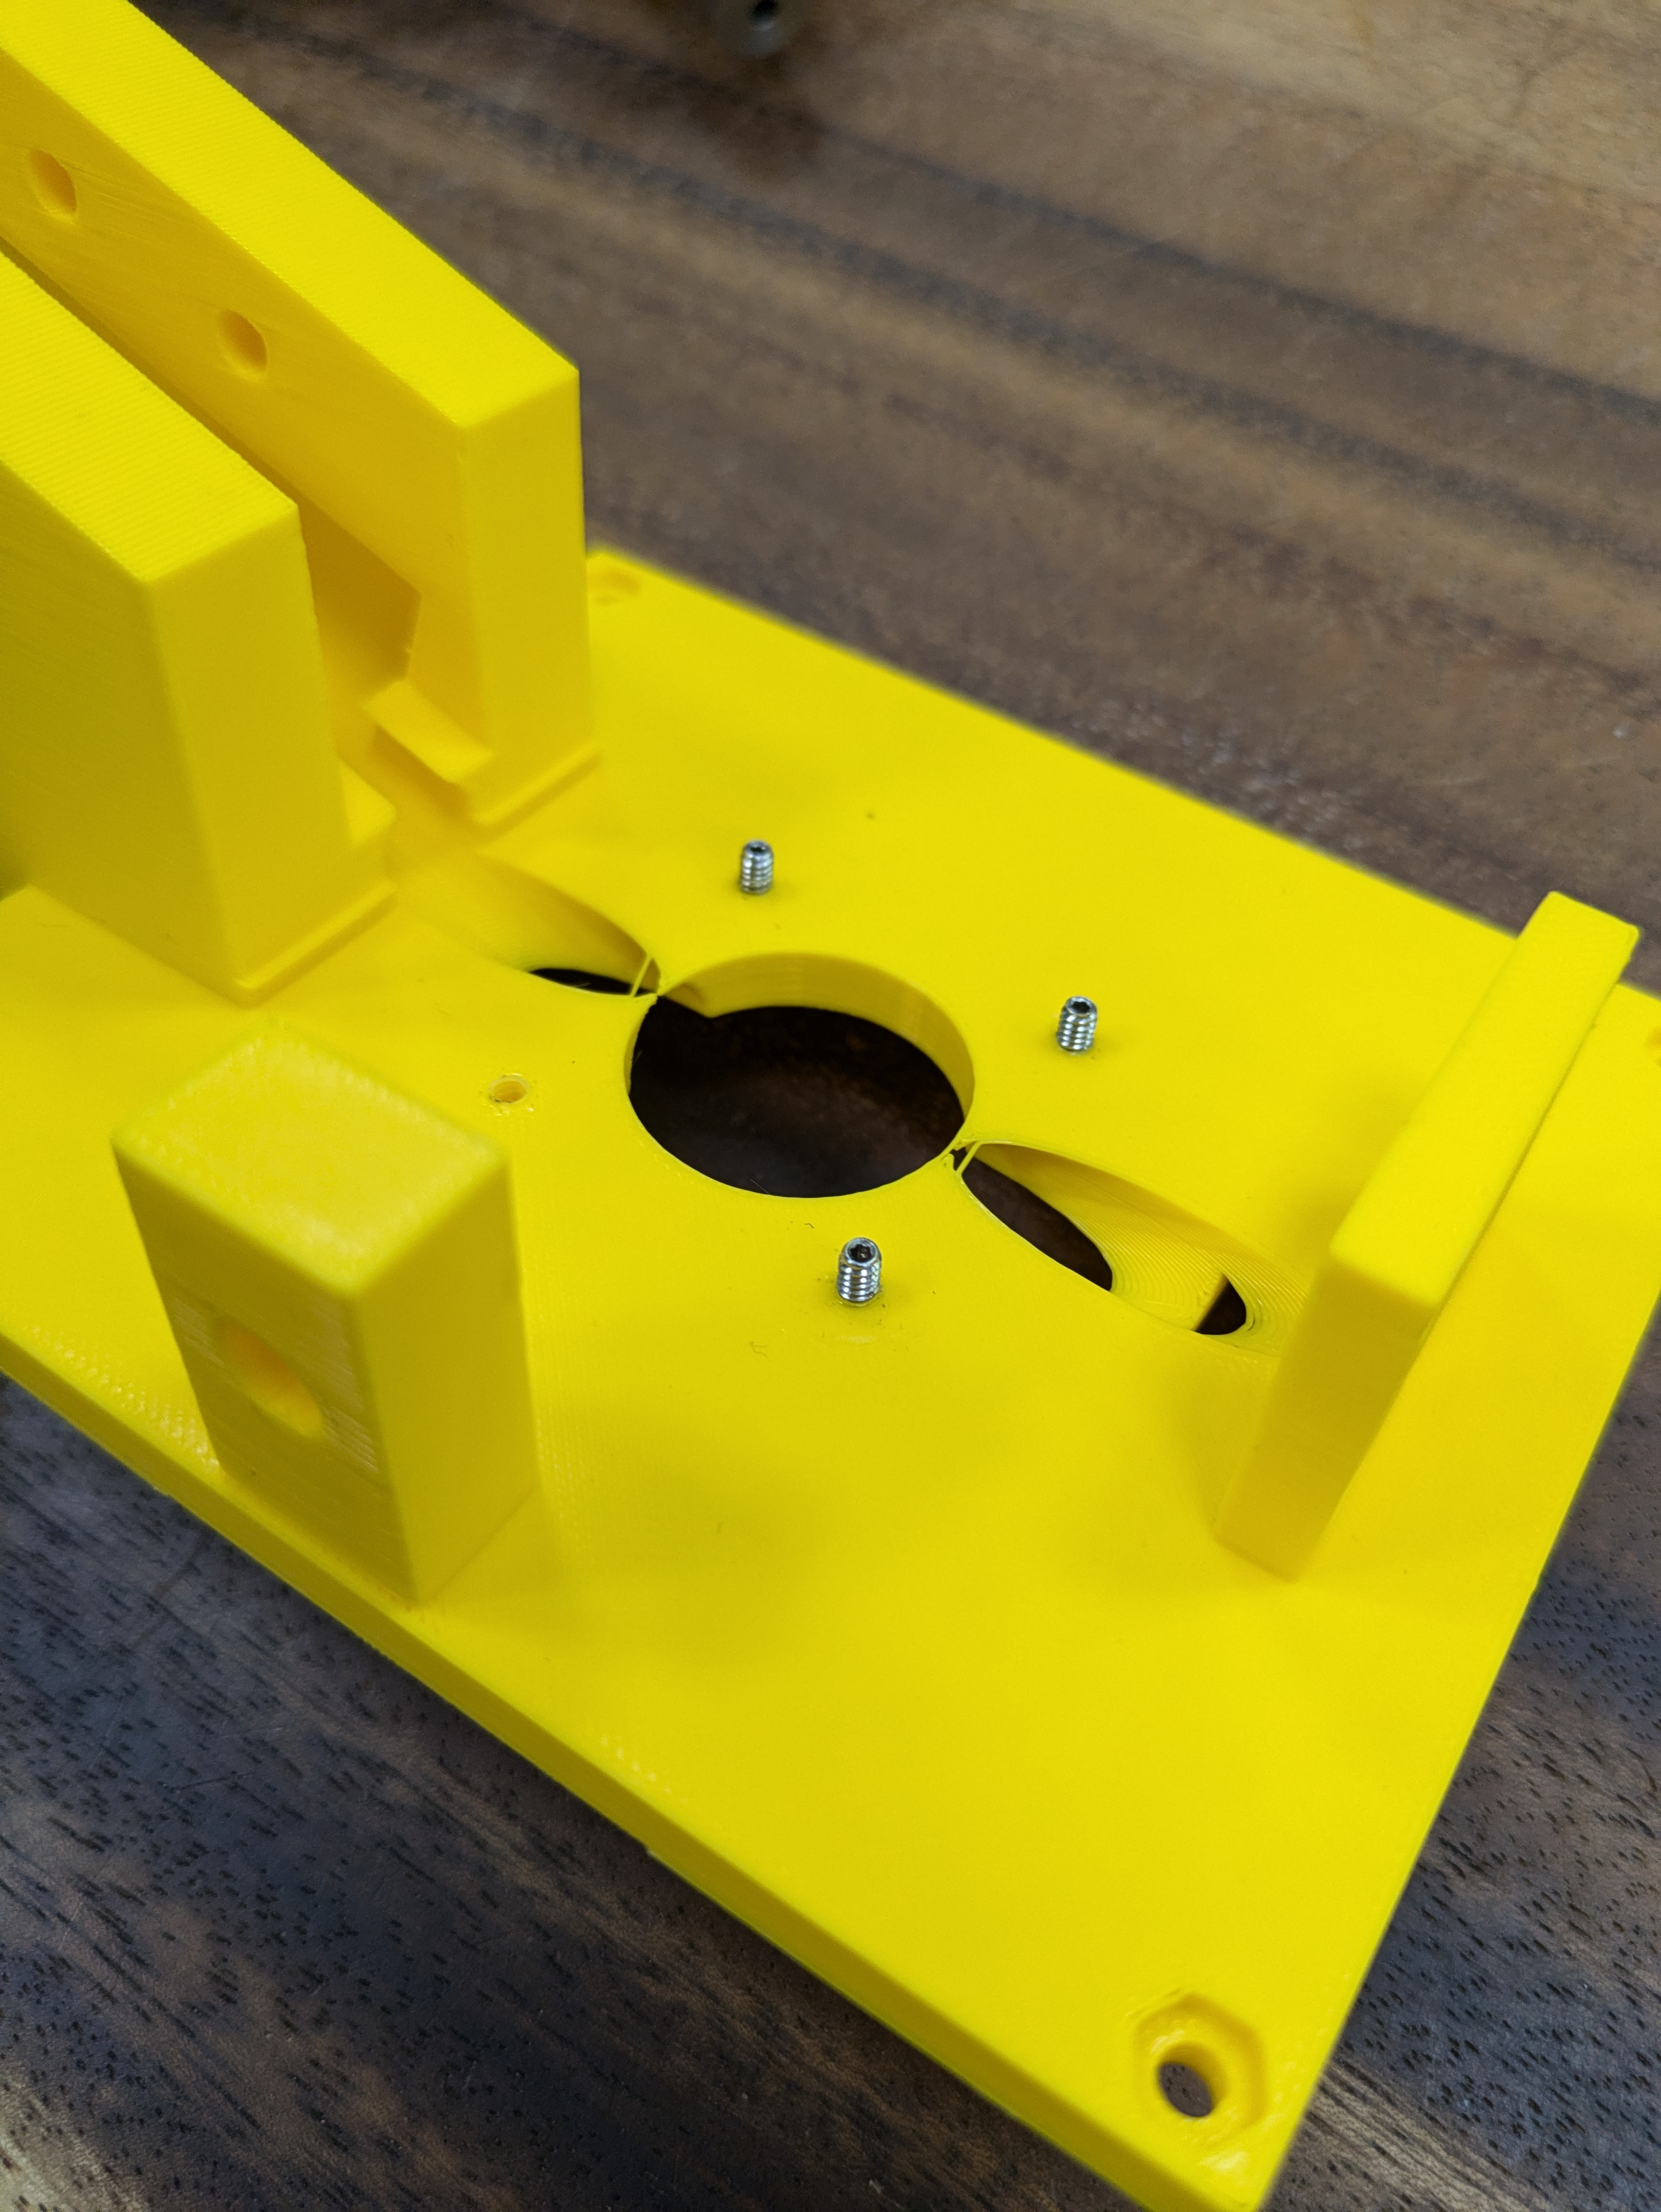
\includegraphics[width=\linewidth]{images/boltplacement.jpg}
        \caption{Olympus Stage bolt placement}
        \label{fig:olympus_bolt_placement}
    \end{minipage}
    \hfill
    \begin{minipage}[b]{0.38\textwidth}
        \centering
        \includegraphics[width=\textwidth]{images/} 
        \caption{Main Body with Olympus Stage}
        \label{fig:mainbody&olympus}
    \end{minipage}
\end{figure}

\begin{wrapfigure}{r}{0.3\textwidth}
    \begin{minipage}{0.3\textwidth}
        \includegraphics[width=\linewidth]{images/.png}
        \caption{Laser Holding Sleeve}
        \label{fig:laser_holder}
        
        \vspace{5mm}

        \includegraphics[width=\linewidth]{images/laser_adjustments.png} 
        \caption{Laser Adjustment Bolts}
        \label{fig:laser_adjustments}
    \end{minipage}
\end{wrapfigure}

To thread the cage assembly rods onto the 4-40 bolts, make sure that all the rods spin freely and then thread them onto the bolts in the stage. Since the magnifying lens will be moving freely too, be careful to keep it raised in place if you put the main body of the microscope upside down to more easily thread the cage assembly rods onto the bolts. 

Lastly, place the ThorLab KADF11 laser inside the laser holder and tighten the laser holding sleeve onto the laser by passing two M3 bolts through the side holes of the laser holder and tightening a nut to each bolt, as shown in \ref{fig:laser_holder}. Be careful to point the laser close to the center of the stage opening as you tighten the laser holder, more precise adjustments can later be realised by turning the adjustment bolts built into the laser, shown in \ref{fig:laser_adjustments}.

\subsection{Mounting the Base and Sample Holder}

It is not a great time to mount the cage system on the base as shown in figure \ref{fig:microscope_on_base}. This will allow easier access to the four eyelets at the corners of the Olympus Stage. To secure the sample holder to the Olympus stage, insert four M3 bolts through the eyelets in the sample holder and then thread four nuts to the bolts under the Olympus Stage. Once these nuts are tightened, the microscope is complete, see \ref{fig:complete_microscope}. 

\begin{figure}
    \centering
    \begin{minipage}[b]{0.5\textwidth}
        \includegraphics[width=0.45\linewidth]{images/}
        \caption{Main Body with Olympus on Base}
        \label{fig:microscope_on_base}
    \end{minipage}
    \hfill
    \begin{minipage}[b]{0.5\textwidth}
        \includegraphics[width=0.45\linewidth]{images/}
        \caption{Final Set-Up}
        \label{fig:complete_microscope}
    \end{minipage}
\end{figure}



\end{document}
